% Copyright (c) 2015 Benito Palacios Sánchez - All Rights Reserved.
% Esta obra está licenciada bajo la Licencia Creative Commons Atribución 4.0
% Internacional. Para ver una copia de esta licencia, visita
% http://creativecommons.org/licenses/by/4.0/.

\section[Contenido con copyright]{Contenido con derechos de autor}
\subsection{Libros electrónicos}
\begin{frame}{Ninokuni: La ira de la Bruja Blanca}
\begin{columns}
    \begin{column}{0.65\textwidth}
    \begin{wideitemize}
        \item<1-> Versión para PS3 con ligeros cambios. Llegó a América y Europa.

        \item<2-> Libro digitalizado en alta calidad.

        \item<3-> No hay algoritmos de protección, pero su formato no es estándar.
        \begin{itemize}
            \item<4-> El resto de ficheros (texto, audio, etc) sí están cifrados.
            \note<1>[item]{El cifrado es nativo de la consola.}
        \end{itemize}
    \end{wideitemize}
    \end{column}

    \begin{column}{0.35\textwidth}
        \visible<2->{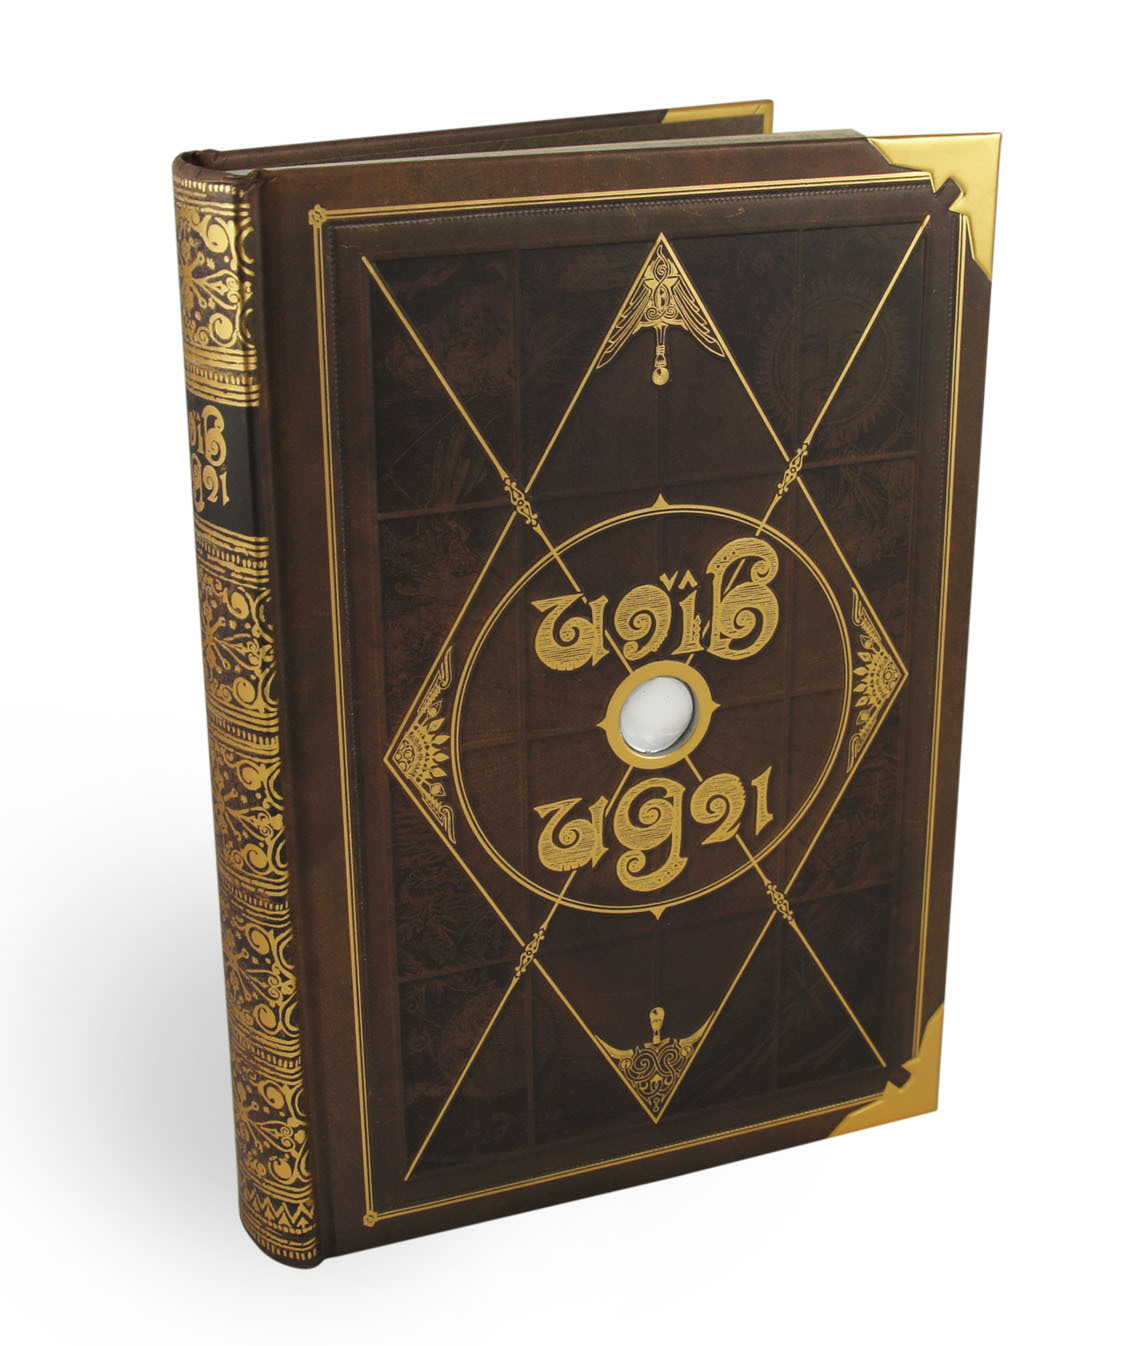
\includegraphics[width=\textwidth,keepaspectratio]{imgs/nino_book.jpg}}
    \end{column}

\end{columns}
\end{frame}

\subsection{Bandas sonoras}
\begin{frame}{Guitar Hero: On Tour}

\begin{columns}
    \begin{column}{0.35\textwidth}
        \visible<1->{
\includegraphics[width=\textwidth,keepaspectratio]{imgs/guitar_grip.png}}
    \end{column}

    \begin{column}{0.65\textwidth}
    \begin{wideitemize}
        \item<1-> Ficheros comprimidos con formato propietario.
        \begin{itemize}
            \item<2-> El algoritmo ocupa 1.900 instrucciones máquina.
            \note<1>[item]{Se compiló en modo depuración por los errores.}
        \end{itemize}

        \item<3-> No hay compresión en las siguientes ediciones.

        \item<4-> Canciones en formato \texttt{Vorbis OGG}.
    \end{wideitemize}
    \end{column}
\end{columns}

\vfill
\visible<2->{\includefigure{Mensajes de error en el código.}{imgs/zlib_debug.png}}
\note<1>[item]{Al incluir hardware adicional no se puede piratear.}
\note<1>[item]{Se creó un parche para eliminar la dependencia de hardware.}

\end{frame}

\begin{frame}{Duet}
\begin{columns}
    \begin{column}{0.75\textwidth}
    \begin{center}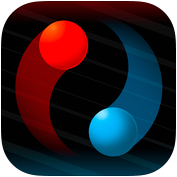
\includegraphics[width=0.15\textwidth,keepaspectratio]{imgs/duet_logo.png}\end{center}

    \begin{wideitemize}
        \item<1-> Juego para plataformas móviles (Android, iOS).

        \item<2-> La banda sonora se vende en iTunes por 3.99€.

        \item<3-> Se encuentra desprotegida en la carpeta del juego en formato estándar.
    \end{wideitemize}
    \end{column}

    \begin{column}{0.25\textwidth}
        \centering
        \visible<3->{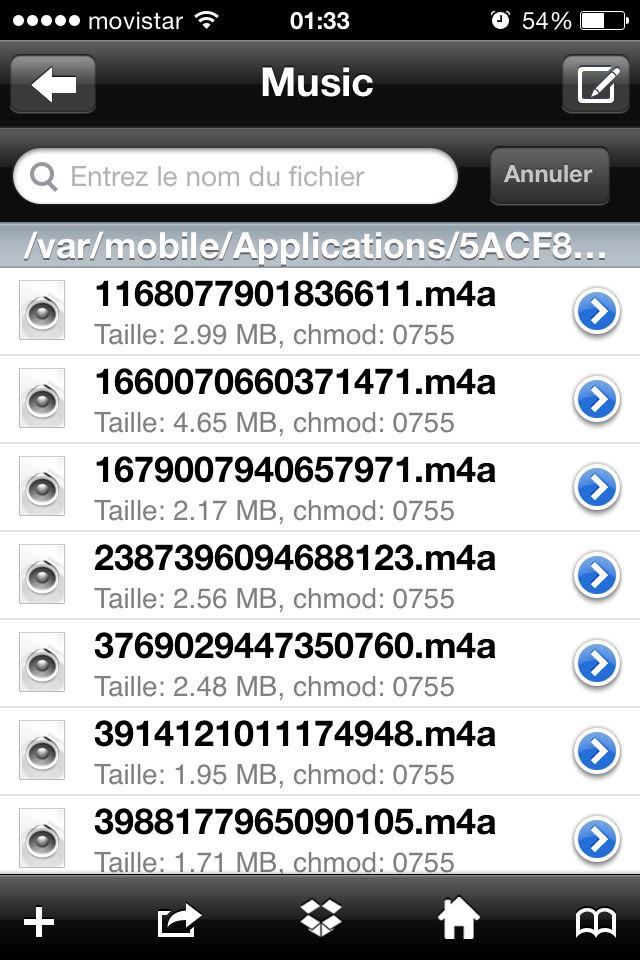
\includegraphics[width=\textwidth,keepaspectratio]{imgs/duet_music.png}}
    \end{column}
\end{columns}
\end{frame}

\subsection{}
\begin{frame}{Mecanismos en otros juegos}
Información en otros juegos estudiados:

\begin{wideitemize}
    \item<+-> \textit{100 Classic Book Collection}: Sin protección en \textit{e-books}. \textcolor{BrickRed}{\ding{53}}

    \item<+-> \textit{Elite Beat Agents}: Sin protección en canciones. \textcolor{BrickRed}{\ding{53}}

    \item<+-> \textit{Guitar Rock}: Sin protección en canciones. \textcolor{BrickRed}{\ding{53}}

    \item<+-> Música de juegos de Level-5: Codificación propietaria. \textcolor{OliveGreen}{\ding{51}}

    \item<+-> Vídeos de \textit{Ninokuni} para PS3: Codificación \texttt{MPEG}. \textcolor{BrickRed}{\ding{53}}

    \item<+-> Vídeos en NDS: Codificación propietaria desconocida. \textcolor{OliveGreen}{\ding{51}}
\end{wideitemize}
\end{frame}
